%Copyright 2014 Jean-Philippe Eisenbarth
%This program is free software: you can 
%redistribute it and/or modify it under the terms of the GNU General Public 
%License as published by the Free Software Foundation, either version 3 of the 
%License, or (at your option) any later version.
%This program is distributed in the hope that it will be useful,but WITHOUT ANY 
%WARRANTY; without even the implied warranty of MERCHANTABILITY or FITNESS FOR A 
%PARTICULAR PURPOSE. See the GNU General Public License for more details.
%You should have received a copy of the GNU General Public License along with 
%this program.  If not, see <http://www.gnu.org/licenses/>.

%Based on the code of Yiannis Lazarides
%http://tex.stackexchange.com/questions/42602/software-requirements-specification-with-latex
%http://tex.stackexchange.com/users/963/yiannis-lazarides
%Also based on the template of Karl E. Wiegers
%http://www.se.rit.edu/~emad/teaching/slides/srs_template_sep14.pdf
%http://karlwiegers.com
\documentclass{scrreprt}
\usepackage{listings}
\usepackage{underscore}
\usepackage[bookmarks=true]{hyperref}
\usepackage[utf8]{inputenc}
\usepackage[english]{babel}
\usepackage{CJKutf8}
\usepackage{graphicx}
\usepackage{float}
\usepackage{longtable}

\hypersetup{
    bookmarks=false,    % show bookmarks bar?
    pdftitle={Software Requirement Specification},    % title
    pdfauthor={Jean-Philippe Eisenbarth},                     % author
    pdfsubject={TeX and LaTeX},                        % subject of the document
    pdfkeywords={TeX, LaTeX, graphics, images}, % list of keywords
    colorlinks=true,       % false: boxed links; true: colored links
    linkcolor=blue,       % color of internal links
    citecolor=black,       % color of links to bibliography
    filecolor=black,        % color of file links
    urlcolor=purple,        % color of external links
    linktoc=page            % only page is linked
}%
\def\myversion{1.0 }
\date{}
%\title
\usepackage{hyperref}
\begin{document}
\begin{CJK}{UTF8}{bkai}
\begin{flushright}
    \rule{16cm}{5pt}\vskip1cm
    \begin{bfseries}
        \Huge{SOFTWARE REQUIREMENTS\\ SPECIFICATION}\\
        \vspace{1.9cm}
        for\\
        \vspace{1.9cm}
        $<$FinGer Shopping$>$\\
        \vspace{1.9cm}
        \LARGE{Version \myversion approved}\\
        \vspace{1.9cm}
        Prepared by $<$Rl$>$\\
        \vspace{1.9cm}
        $<$第11組$>$\\
        \vspace{1.9cm}
        \today\\
    \end{bfseries}
\end{flushright}

\tableofcontents
\chapter*{Revision History}
\begin{center}
    \begin{longtable}{|c|c|c|c|}
        \hline
	    Name & Date & Reason For Changes & Version\\
        \hline
	    俊傑 & 18/06/03 & 建立main form、form4,5,6 & 1.0\\
        \hline
	    家賢 & 18/06/03 & 建立form 2 & 1.1\\
        \hline
	    家賢 & 18/06/03 & 修改form4 & 1.3\\
        \hline
	    俊傑 & 18/06/03 & 修改form的問題 & 1.4\\
        \hline
	    家賢 & 18/06/03 & 新增mongodb和insert & 1.5\\
        \hline
	    俊傑 & 18/06/04 & 新增登入錯誤偵測 & 1.6\\
        \hline
	    家賢 & 18/06/04 & 修改mongodb型態 & 1.7\\
        \hline
	    俊傑 & 18/06/04 & 修改form6顯示username & 1.8\\
        \hline
	    家賢 & 18/06/05 & Form6可以讀取照片 & 1.9\\
        \hline
	    俊傑 & 18/06/05 & add form7(modify password) & 2.0\\
        \hline
	    家賢 & 18/06/05 & 密碼防呆機制 & 2.1\\
        \hline
	    家賢 & 18/06/05 & 資料庫可存放資料 & 2.2\\
        \hline
	    俊傑 & 18/06/06 & 銷售介面新增商品 & 2.4\\
        \hline
	    家賢 & 18/06/06 & 新增form8,9 & 2.5\\
        \hline
	    俊傑 & 18/06/07 & 購買介面新增”售完” & 2.6\\
        \hline
	    宜叡 & 18/06/07 & 實作socket連線Server/Client登入部分 & 2.7\\
        \hline
	    家賢 & 18/06/07 & 新增訂單資料庫 & 2.8\\
        \hline
	    家賢 & 18/06/07 & 新增BugDB function & 2.9\\
        \hline
	    宜叡 & 18/06/07 & add SocketClient.cs & 3.0\\
        \hline
	    俊傑 & 18/06/07 & 新增搜尋功能 & 3.1\\
        \hline
	    家賢 & 18/06/08 & 新增訂單查詢頁面及功能 & 3.2\\
        \hline
	    宜叡 & 18/06/08 & 修改購買商品按鈕罷工、搜尋語法更改 & 3.3\\
        \hline
	    家賢 & 18/06/08 & 新增通知 & 3.5\\
        \hline
	    俊傑 & 18/06/09 & 通知亮燈完成 & 3.6\\
        \hline
	    俊傑 & 18/06/11 & 新增留言button & 3.7\\
        \hline
	    宜叡 & 18/06/11 & 新增BaseDB來處理對資料庫的查詢與新增 & 3.8\\
        \hline
	    家賢 & 18/06/12 & 新增留言DB,但有Bug & 3.9\\
        \hline
	    家賢 & 18/06/12 & 留言板完工 & 4.1\\
        \hline
	    家賢 & 18/06/12 & 在留言板新增賣家顯示 & 4.2\\
        \hline
	    俊傑 & 18/06/13 & 新增評分星星圖示 & 4.3\\
        \hline
	    家賢 & 18/06/13 & 新增評分功能、bug修改完成 & 4.4\\
      \hline
	    冠穎 & 18/06/14 & PPT 初版 & 4.5\\
      \hline
	    宜叡 & 18/06/14 & 更換連接mongoDB的方法 & 4.6\\
      \hline
	    俊傑 & 18/06/14 & 增加評分排序功能 & 4.7\\
      \hline
	    昆毅 & 18/06/14 & PDF初版 & 4.8\\
      \hline
	    宜叡 & 18/06/14 & 更改連線方式 & 4.9\\
      \hline
	    冠穎 & 18/06/15 & 新增 The Intelligent Communication & 5.0\\
      \hline
	    家賢 & 18/06/15 & 新增PDF文件 & 5.1\\
      \hline
	    冠穎 & 18/06/15 & create ppt & 5.2\\
      \hline
	    冠穎 & 18/06/15 & srs 新增程式架構 使用者介面 & 5.3\\
      \hline
	    昆毅 & 18/06/19 & Revision History 完成 & 5.4\\
        \hline
    \end{longtable}
\end{center}

\chapter{介紹}

\section{目的}
\qquad 此文件的目主要在於說明「FinGer Shopping」所規劃的各項功能之軟體設計規格、範圍及參考文件。使用者可透過參考此份文件來了解本系統的架構、環境、作業流程及系統的各項功能,可作為日後軟體設計與軟體測試的依據。

\section{使用者規格書}
\qquad 此規格書提供開發者「FinGer Shopping」內部所制定內容的依據,主要是提供給日後此系統的設計者、開發者與測試者在進行系統開發時的依據,並給此套系統的維護人員來做參考。

\subsection{開發者}
\qquad 開發者可以依照不同的系統的規劃制定特定的功能,也可以依照自己的喜好設定使用者介面,並提供買賣有一個公平透明的交易明台,適時提供買家與賣家相對的服務來改善使用者體驗,並且新增更多功能以提供使用者更強大的服務。

\subsection{買家}
\qquad 對買家而言,可以在文件中找到相對應的功能,並在購買介面並利用搜尋的功能找到自己所需要的目標,並寫在購買之後會提供商品相關的資訊。

\subsection{賣家}
\qquad 對賣家而言,可以在銷售的介面輕鬆上傳自己的商品,並且即時加到販賣的序列提供消費者搜尋選購。若買家購買之後,也會即時跳出有新的訊息的圖示提醒相關的資訊。

\section{涵蓋範圍}
\qquad 此文件的範圍是針對「FinGer Shopping」之軟體需求規格,包括系統前端(C\#)及系統後端(MongoDB)的相關架構與功能。

\section{參考資料}
MongoDB API:http://api.mongodb.com/ \\
C\# 指南:https://docs.microsoft.com/zh-tw/dotnet/csharp/ \\


\chapter{產品描述}

\section{產品願景}
\qquad 在這個網路蓬勃發展的時代,人民對於使用網路可以說是隨手可得。而藉由我們實做出來的交易平台,希望能提供使用者一個簡單且便利買賣
的環境,不僅如此,買家可以輕鬆方便的擔任商品的供給與需求方,更提透明的評分機制,讓使用者可以清楚了解商品的資訊,建立一個隨時隨地都能隨手做買賣的輕鬆便利交易制度。

\section{產品功能}
\qquad FinGer Sopping是一套讓使用者可以同時具備商品的供給與需求方的交易平台。擔任賣家可以透過新增商品同時上傳該商品的圖片、制訂商品價格來銷售自己的商品,並且將會收到來自買方的訂單需求通知;而擔任買家的一方,則可以透過流覽商品來進行選購,若有疑問可以透過商品的評價、或是利用留言版的功能來詢問賣家或其他使用者相關的商品資訊,購買後還能做後續的商品狀態的追蹤。

\section{目標族群}
\qquad FinGer Sopping成立的宗旨主要為讓任何對銷售有興趣的使用者都能賣出自己的商品,平台提供賣方一個輕鬆便利提供商品的制度,達到人人都能在網路上當起大老闆;對於賣方則鎖定對網路相當熟悉的年輕人以及對於購買有強烈欲望的家庭主婦。

\section{開發環境}
\qquad 此專案主要由 C\# 中的 Window Form 來作開發環境,並且以 mongodb 做為資料庫,來儲存用戶的相關資料,成品說明則是由LaTex撰寫而成。

\section{程式架構}
\qquad 使用MongoDB做為資料庫,並統一用BaseDB作為存取資料庫的基礎,再依照各頁面不同的需求來新增不同的class,來在相對應的collection進行一個存取的動作。\\

\begin{figure}
	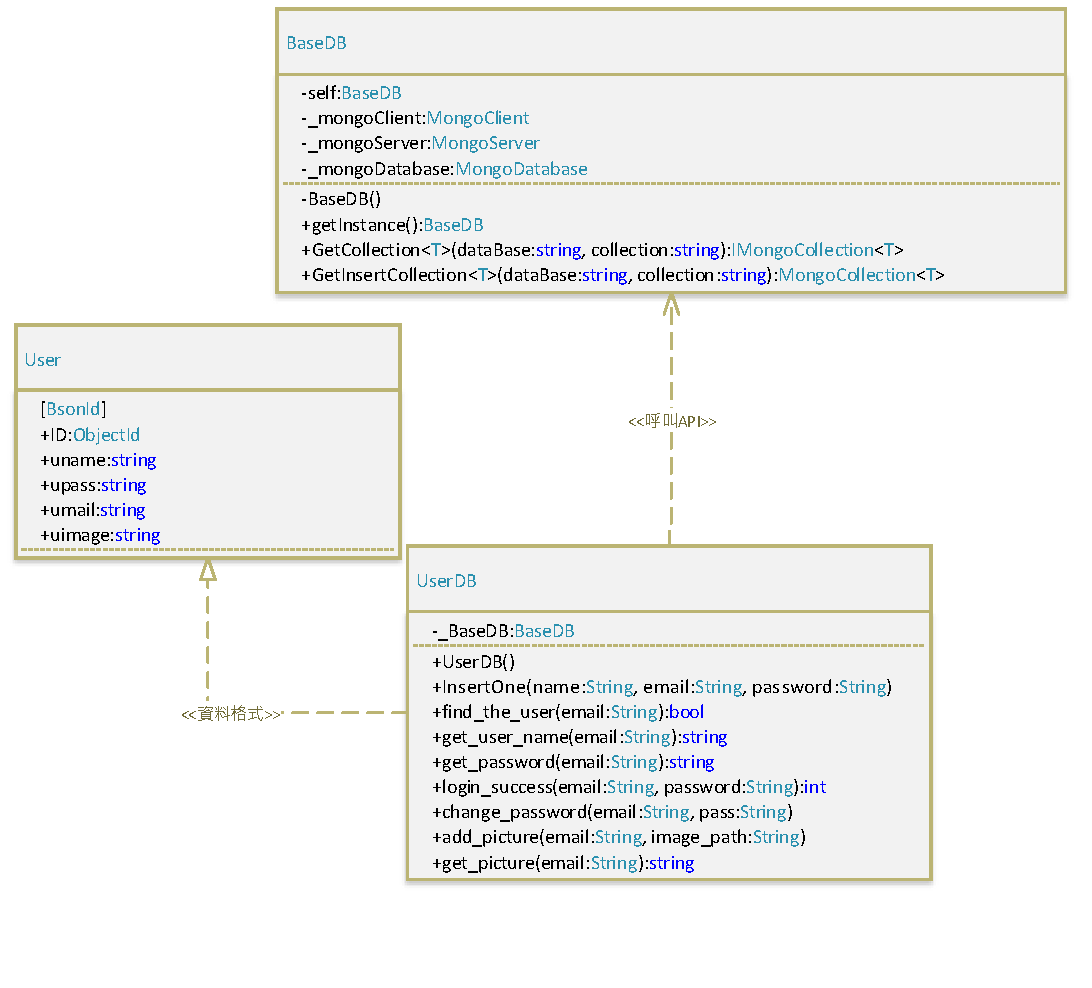
\includegraphics[width=\textwidth]{UserDB.pdf}
	\caption{UserDB用來處理新增、修改使用者登入到資料庫。}
\end{figure}

\begin{figure}
	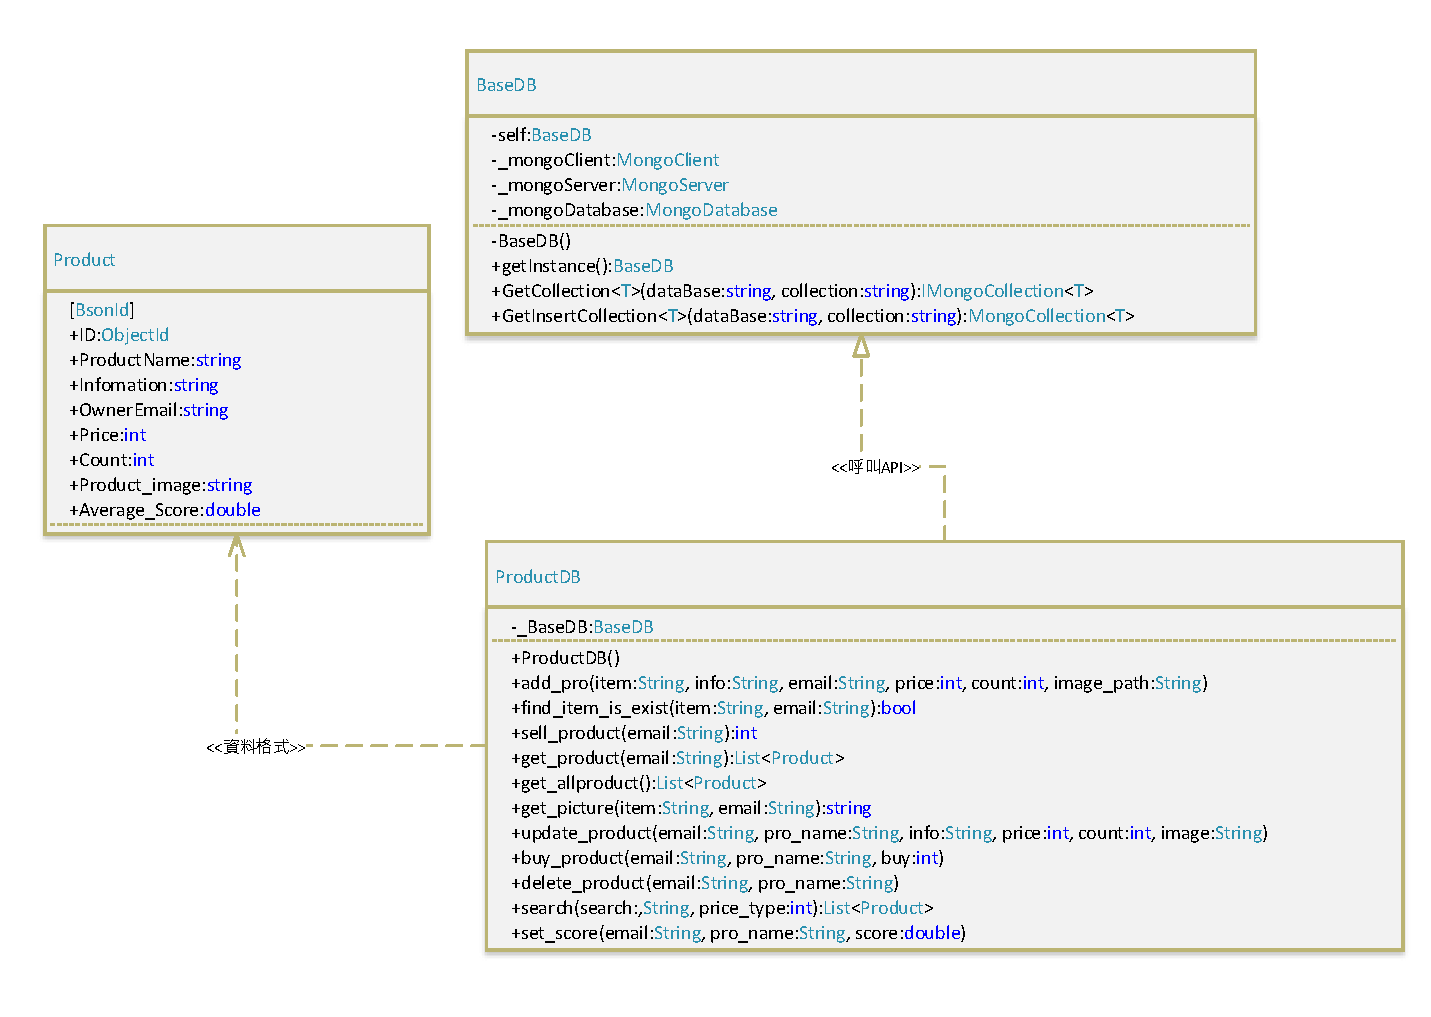
\includegraphics[width=\textwidth]{ProductDB.pdf}
	\caption{ProductDB用來對商品新增、修改、刪除。}
\end{figure}

\begin{figure}
	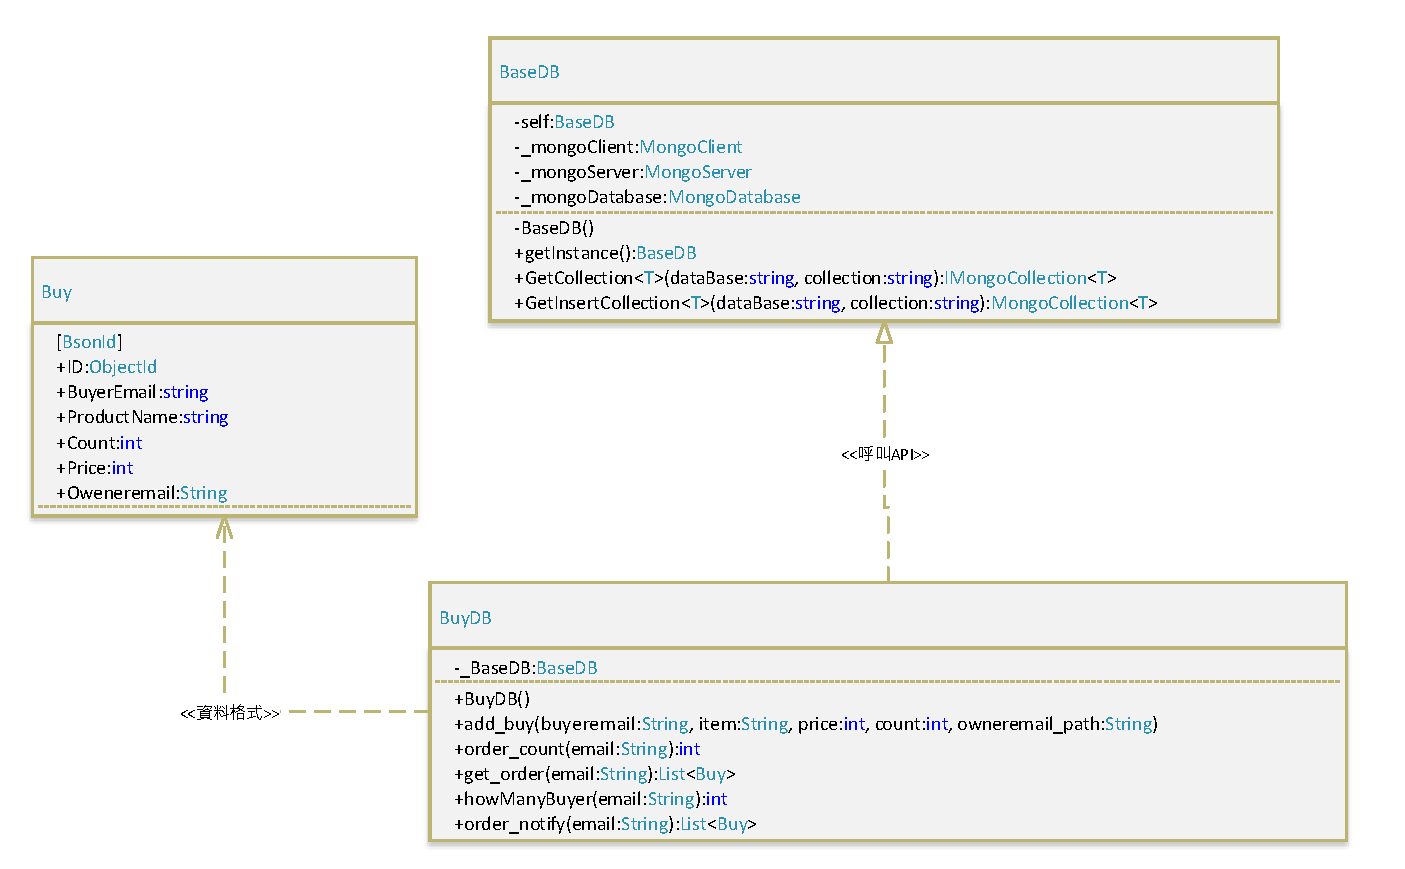
\includegraphics[width=\textwidth]{BuyDB.pdf}
	\caption{BuyDB用來對儲存商品購買紀錄。}
\end{figure}

\begin{figure}
	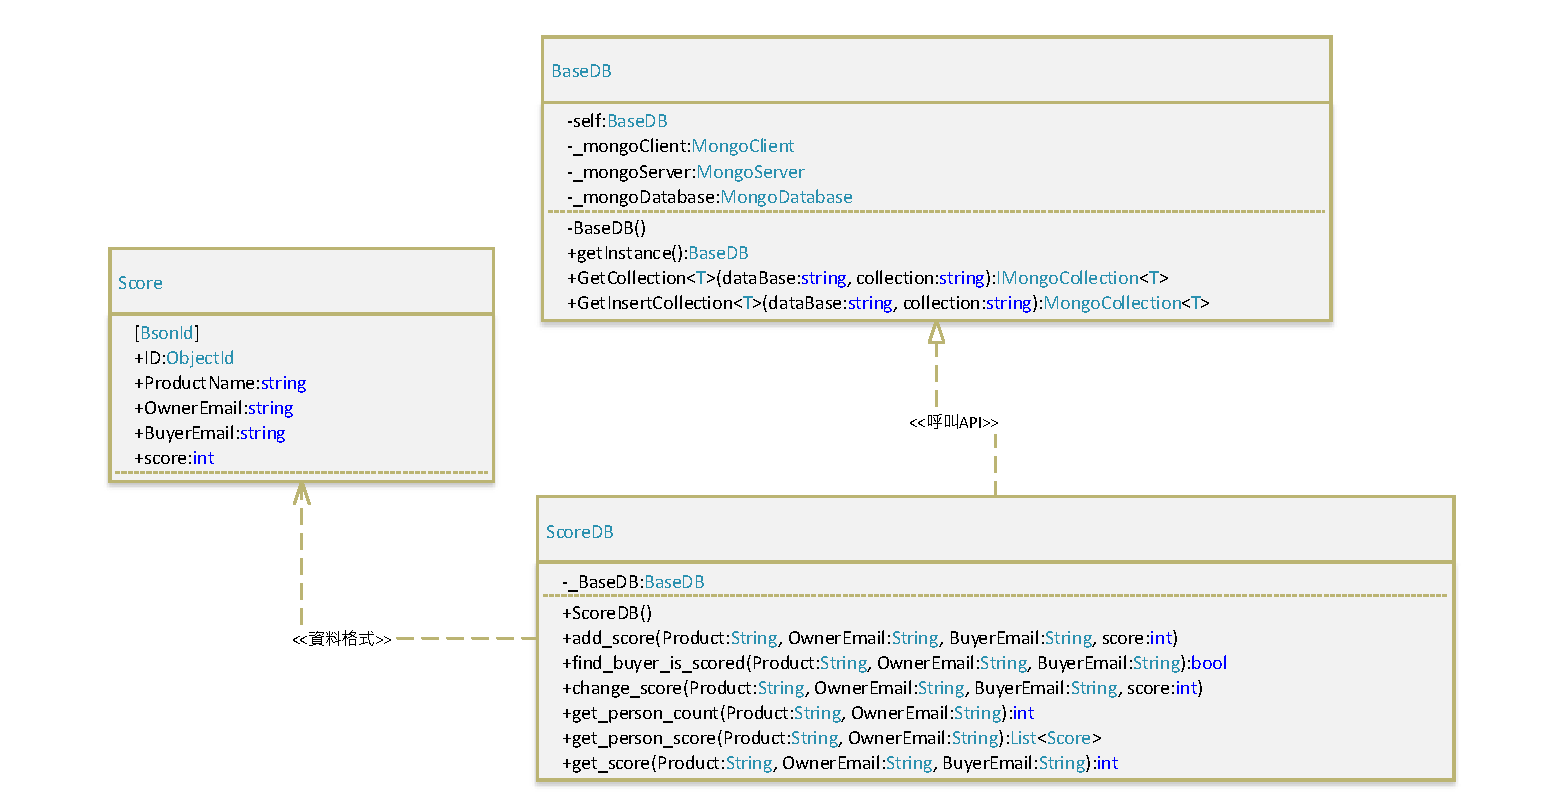
\includegraphics[width=\textwidth]{ScoreDB.pdf}
	\caption{ScoreDB用來紀錄不同使用者對商品的評分。}
\end{figure}

\begin{figure}
	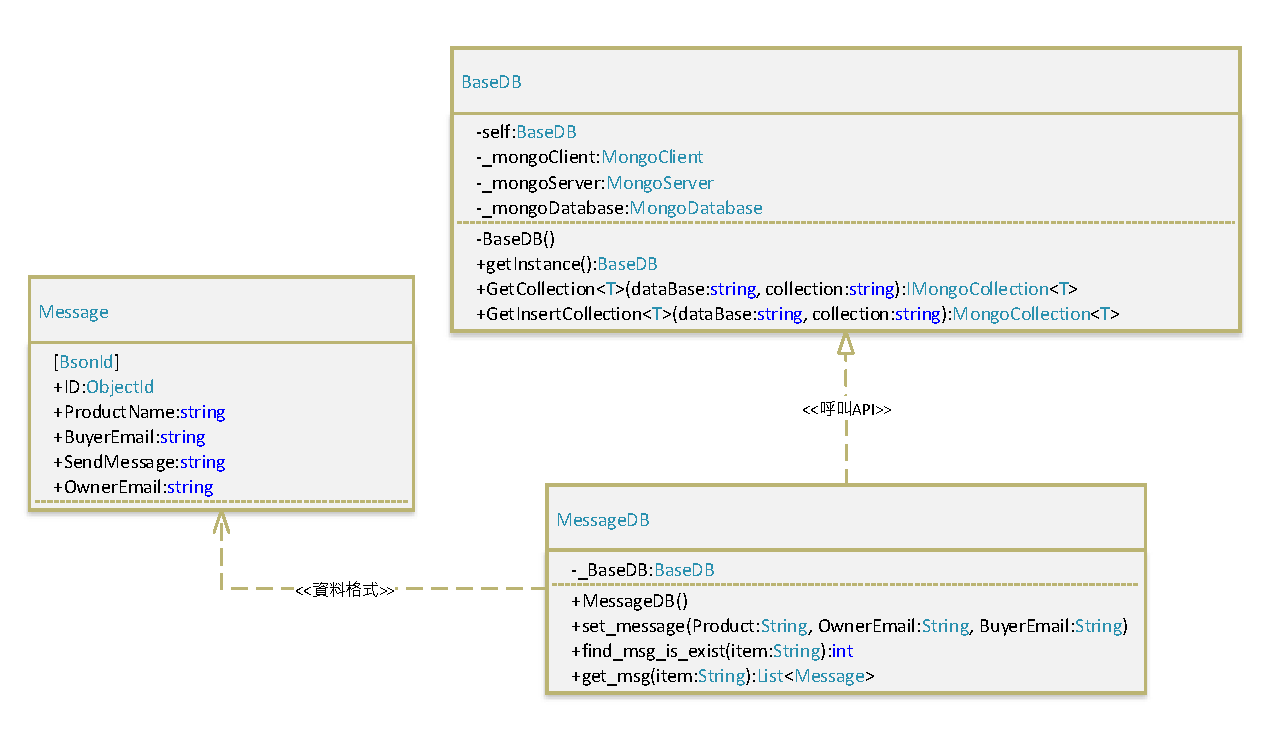
\includegraphics[width=\textwidth]{MessageDB.pdf}
	\caption{MessageDB用來紀錄不同商品使用者對其的留言。}
\end{figure}

\begin{figure}
	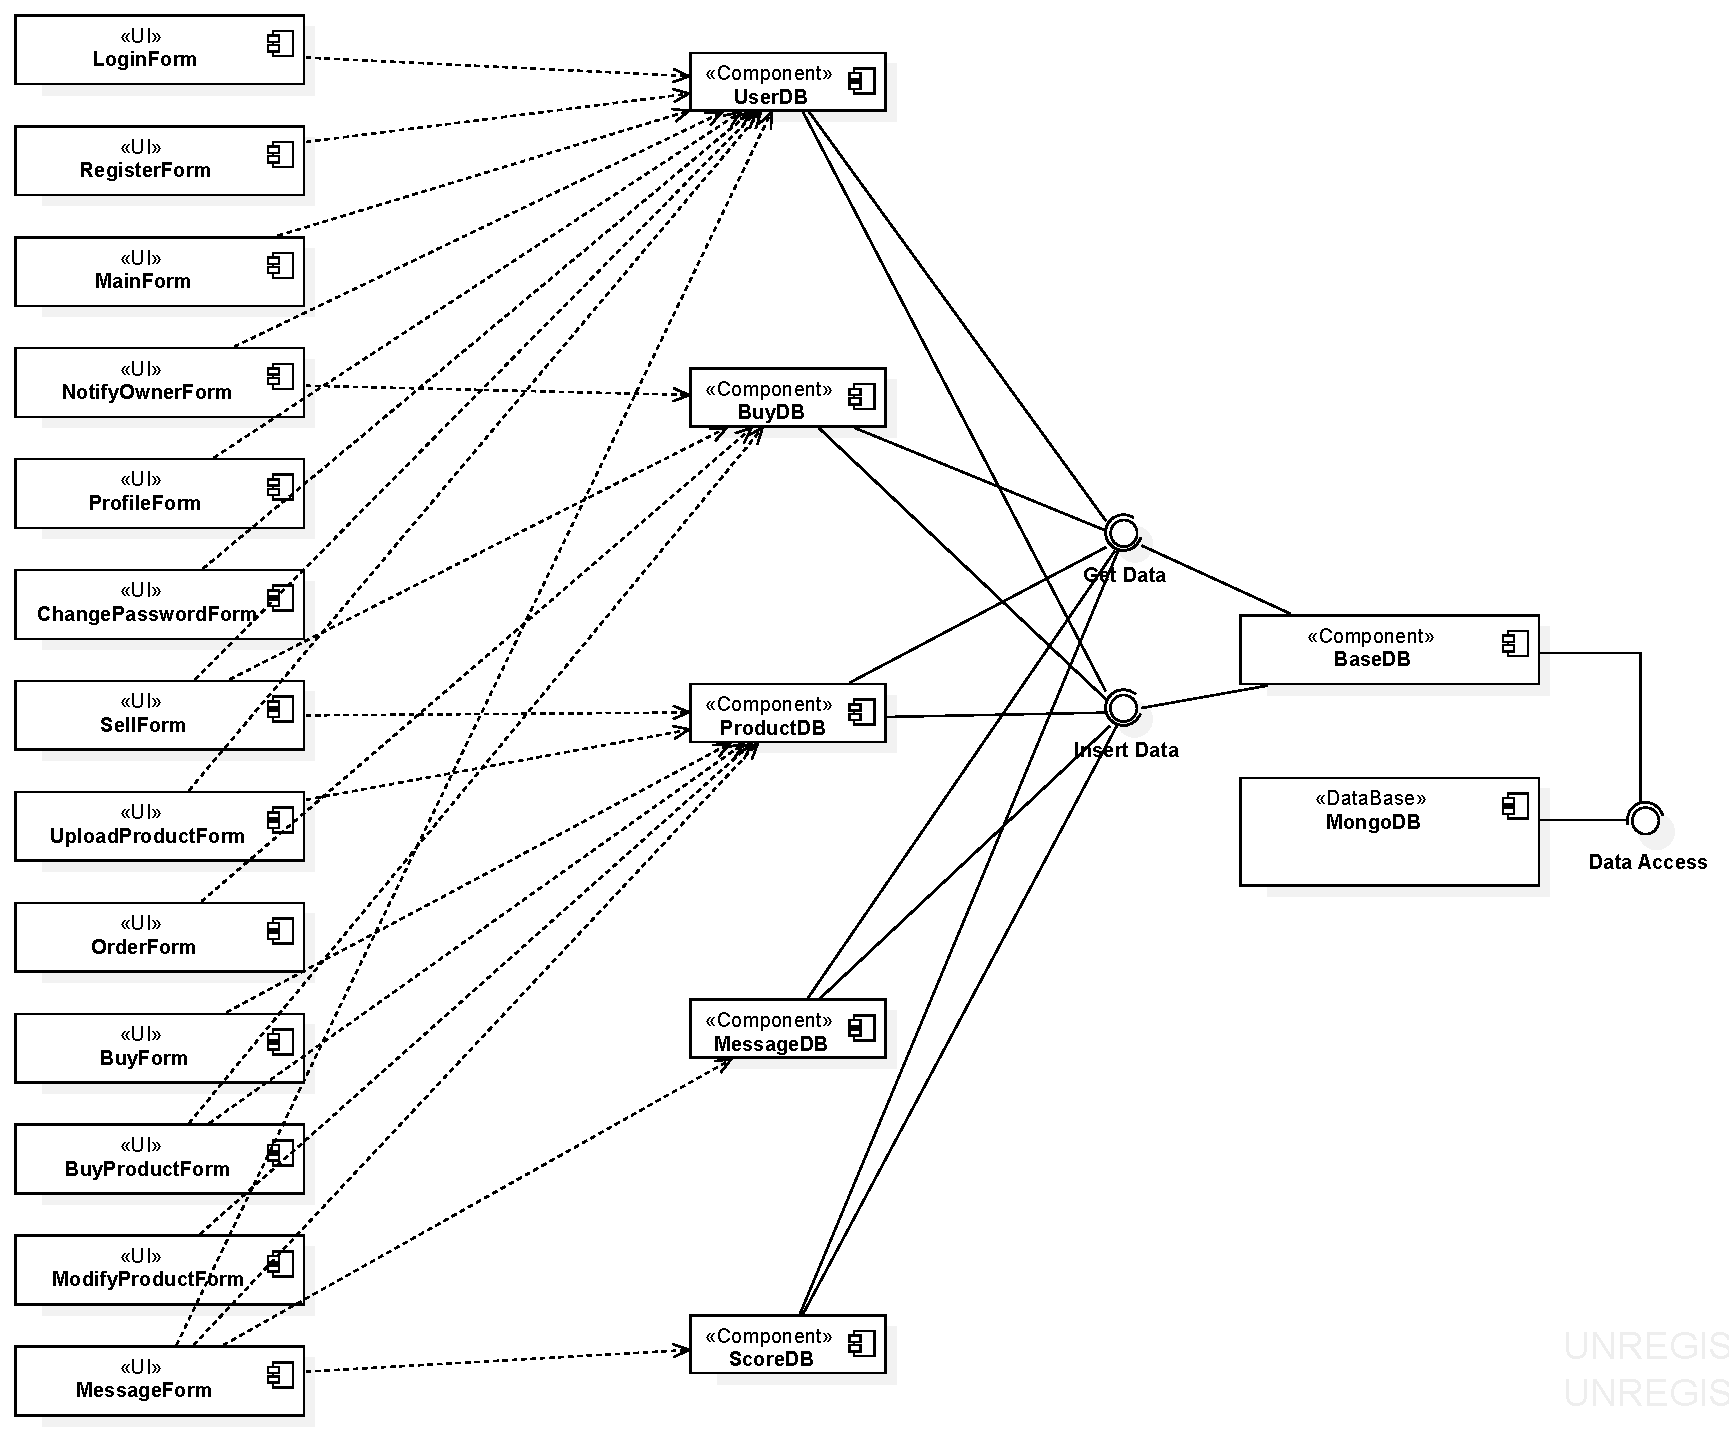
\includegraphics[width=\textwidth]{ComponentDiagram1.pdf}
	\caption{整體的架構。}
\end{figure}


\chapter{External Interface Requirements}

\section{User Interfaces}
\begin{figure}[h]
	\centering
	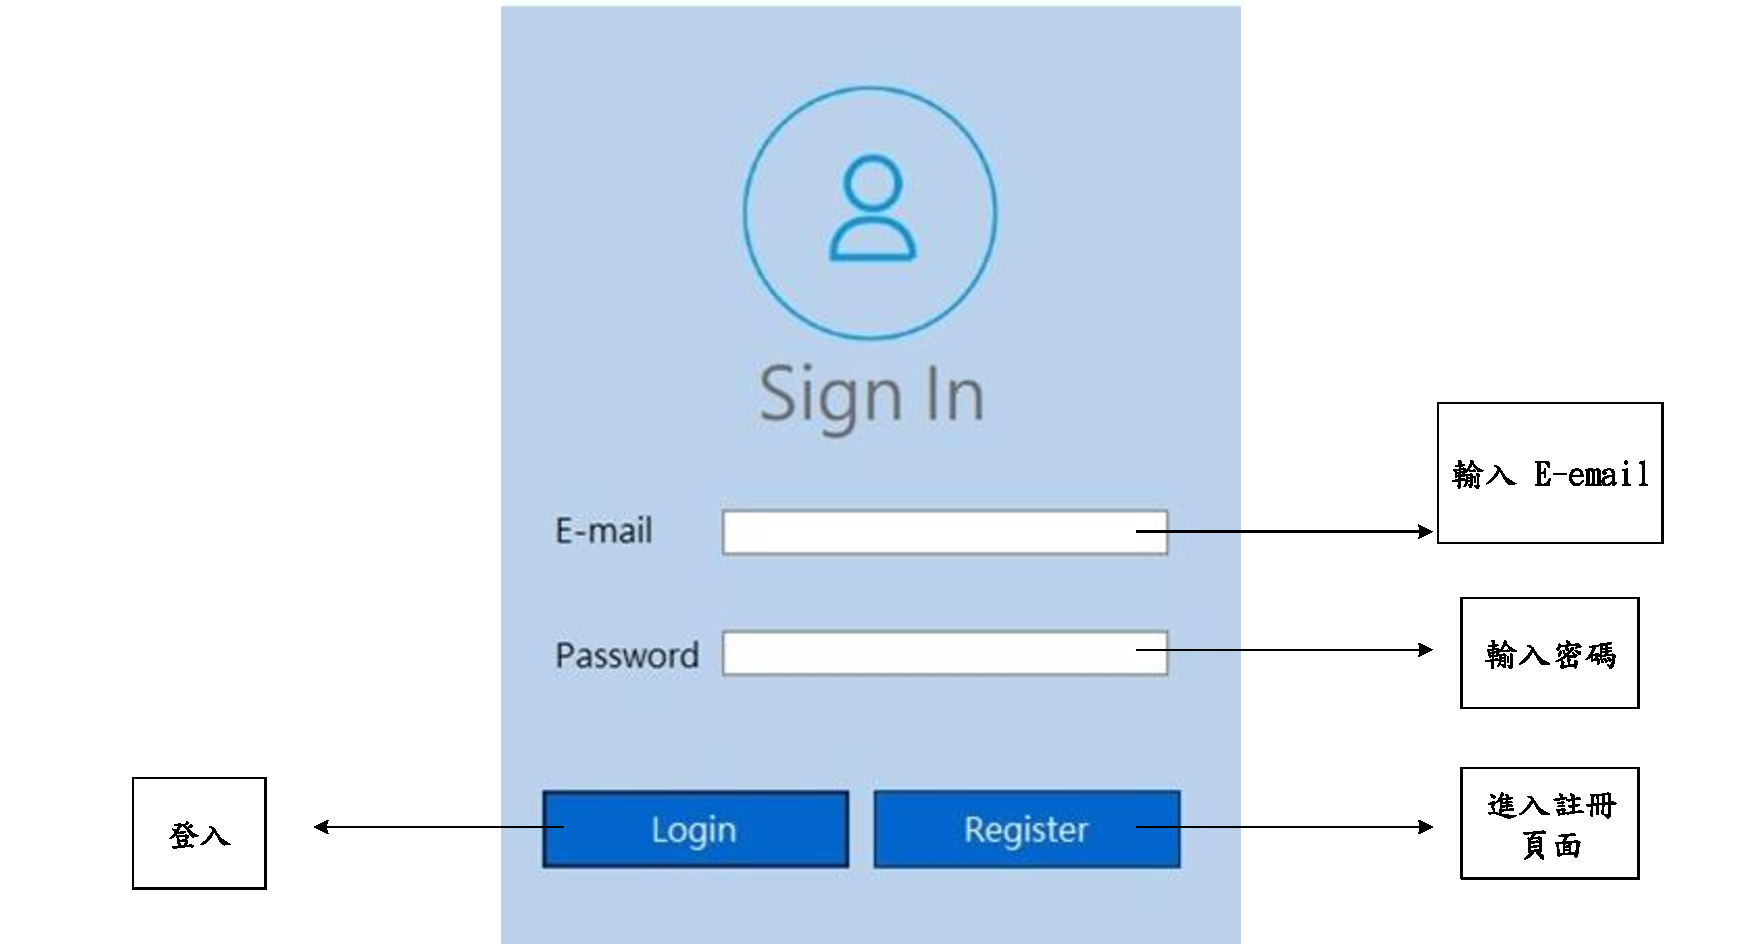
\includegraphics[width=0.85\textwidth]{signin.pdf}
	\caption{登入畫面。}
	\centering
	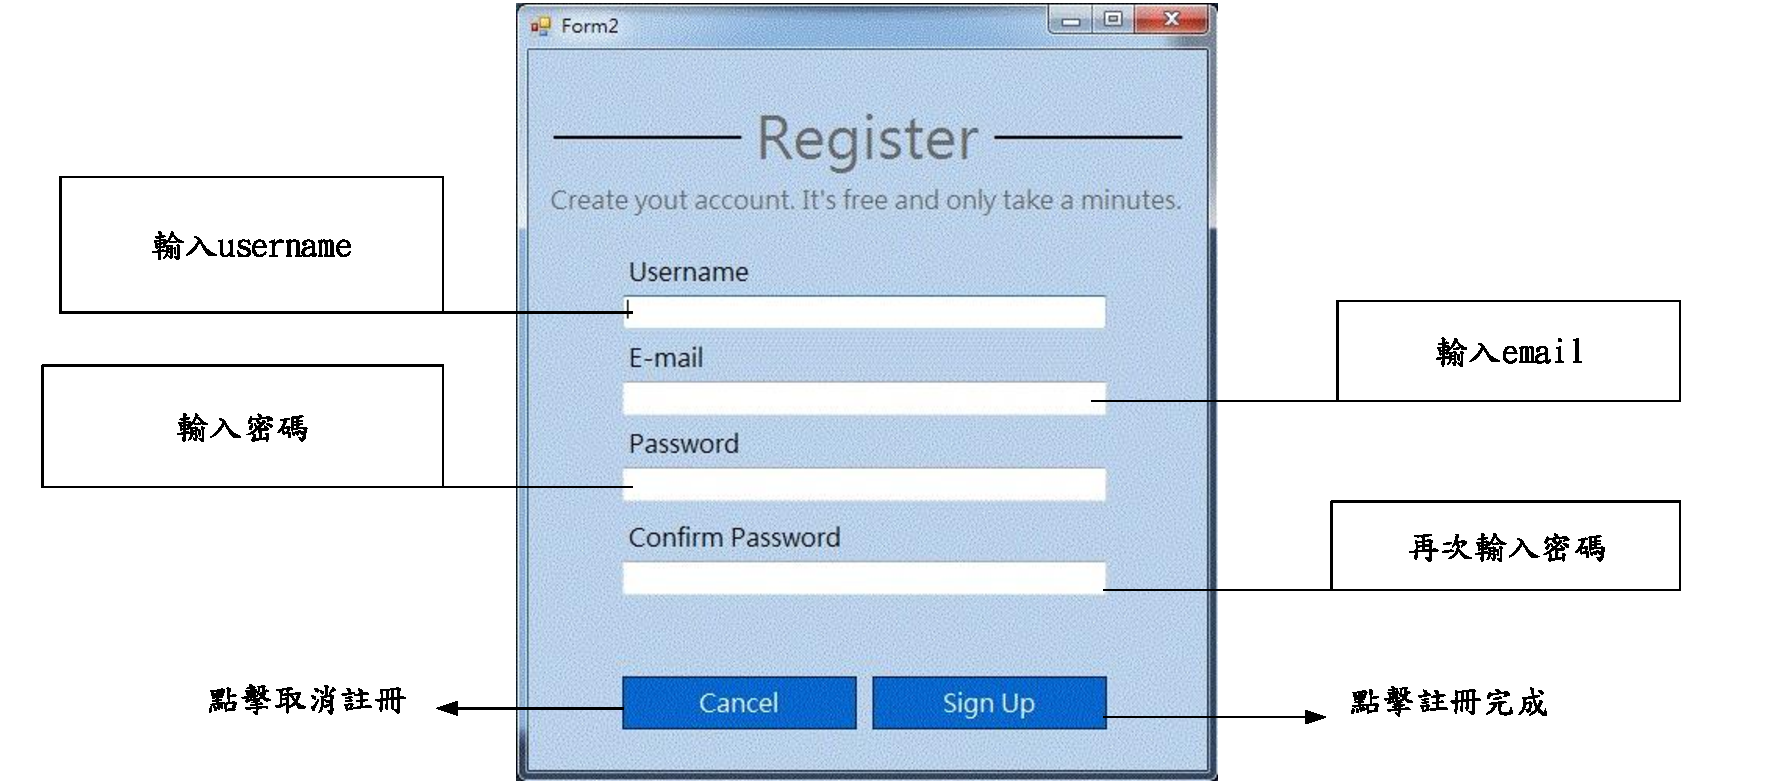
\includegraphics[width=0.85\textwidth]{register.pdf}
	\caption{註冊畫面}
\end{figure}

\begin{figure}[t]
	\centering
	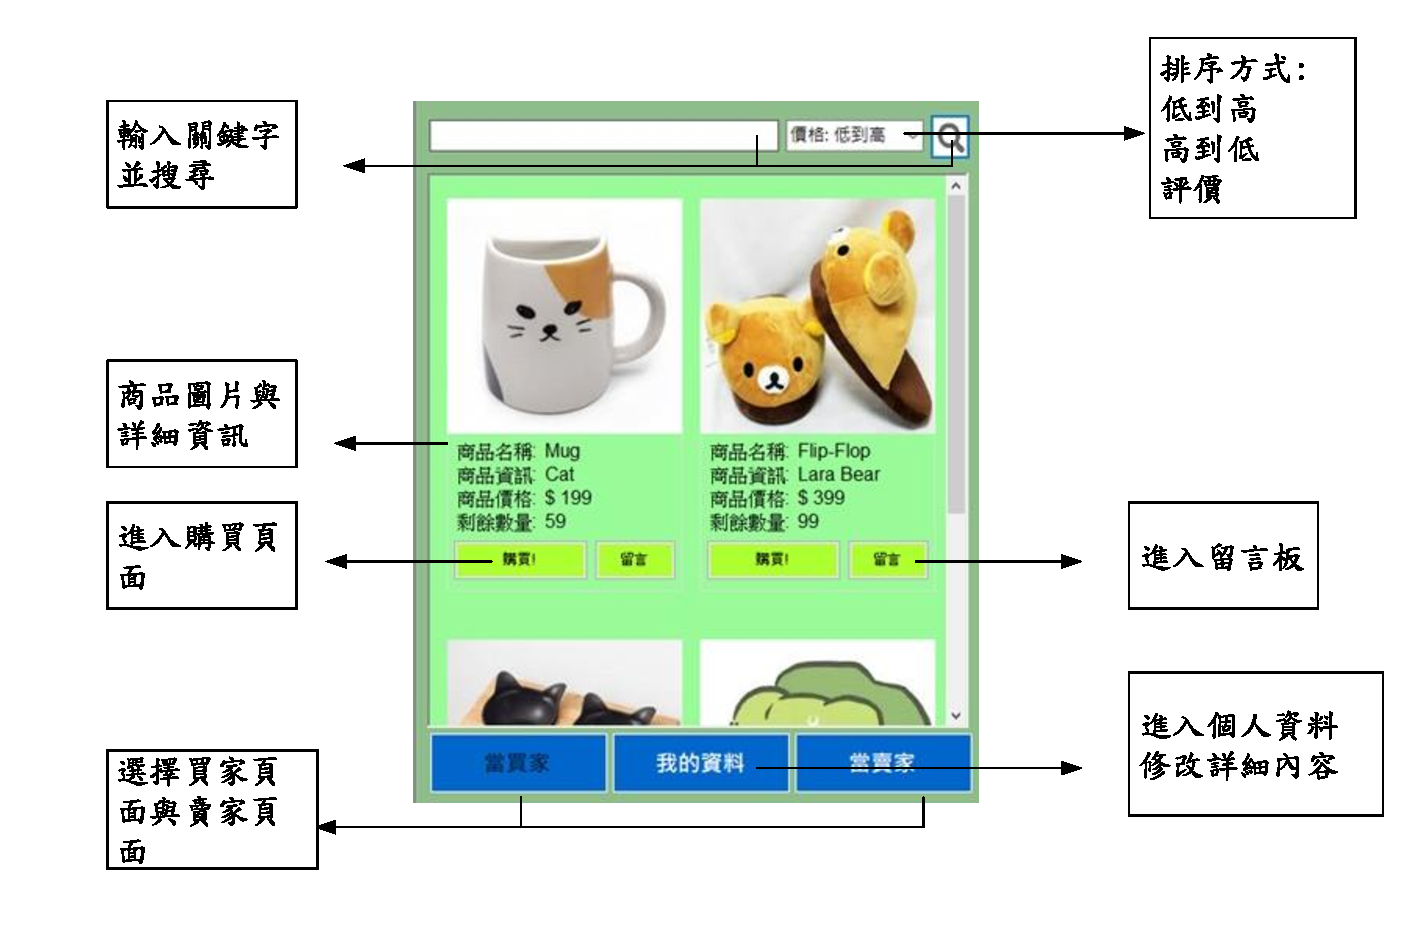
\includegraphics[width=0.85\textwidth]{search.pdf}
	\caption{登入後的頁面,會呈現目前可以買賣的商品。}
	\centering
	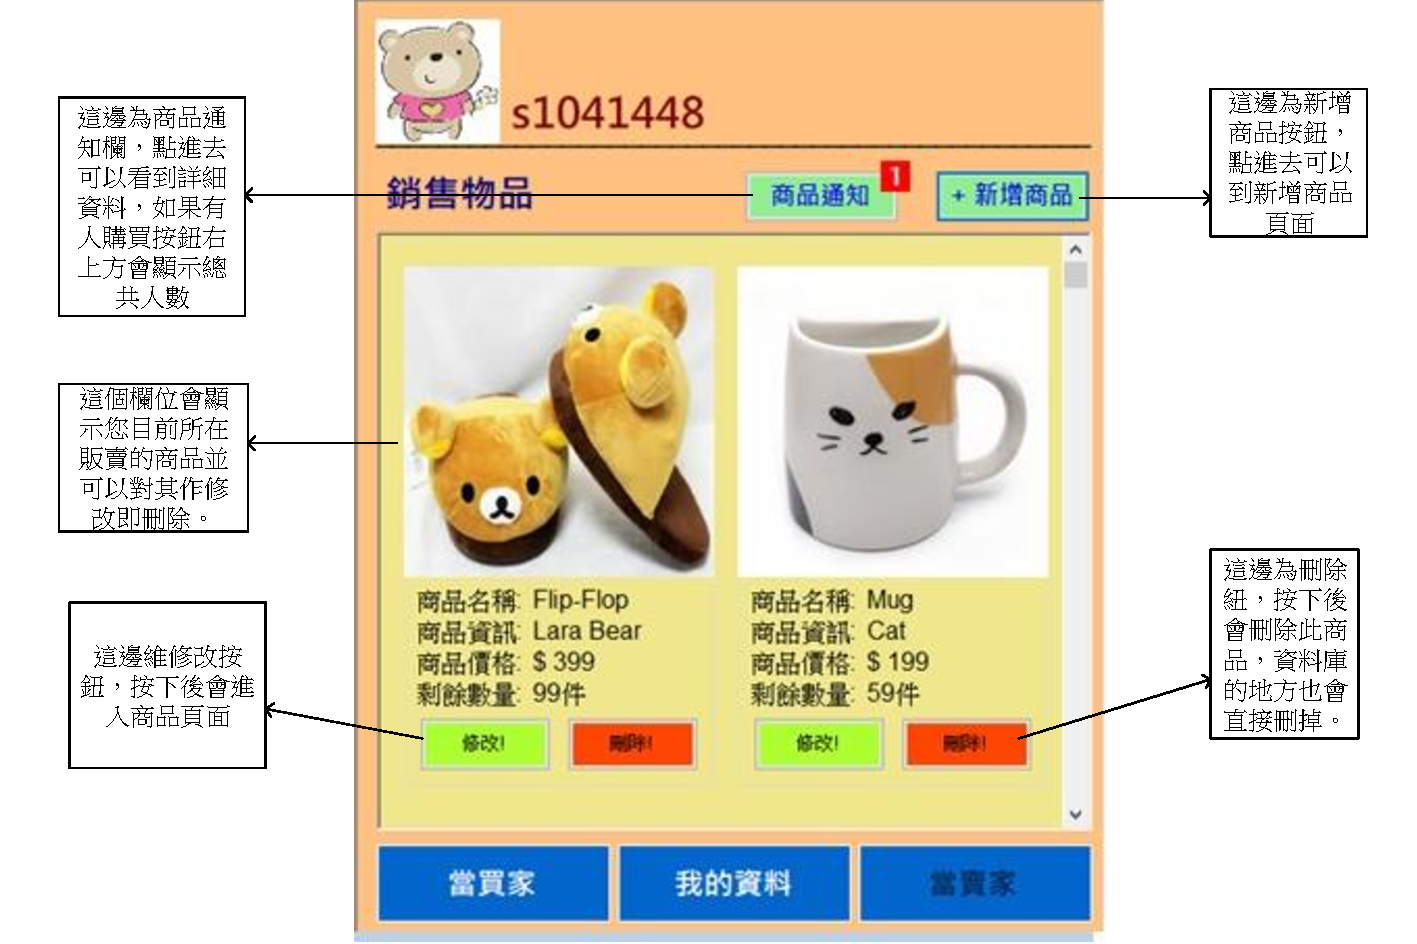
\includegraphics[width=0.85\textwidth]{note.pdf}
	\caption{賣家的畫面。}
\end{figure}

\begin{figure}[t]
	\centering
	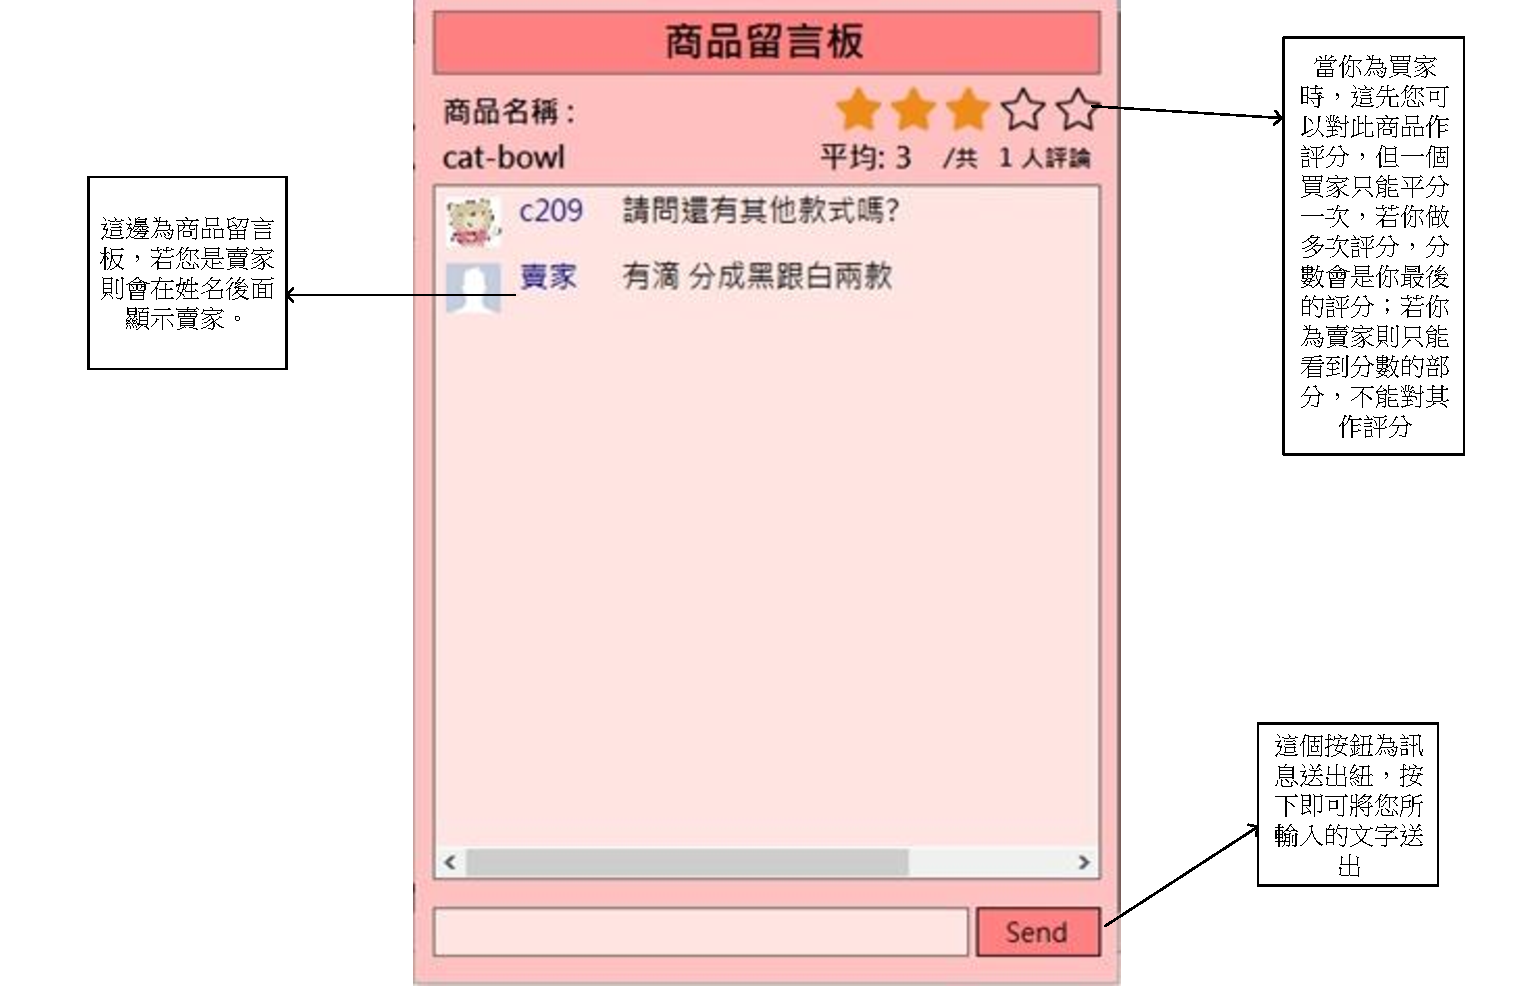
\includegraphics[width=0.80\textwidth]{star.pdf}
	\caption{商品留言和評分頁面。}
	\centering
	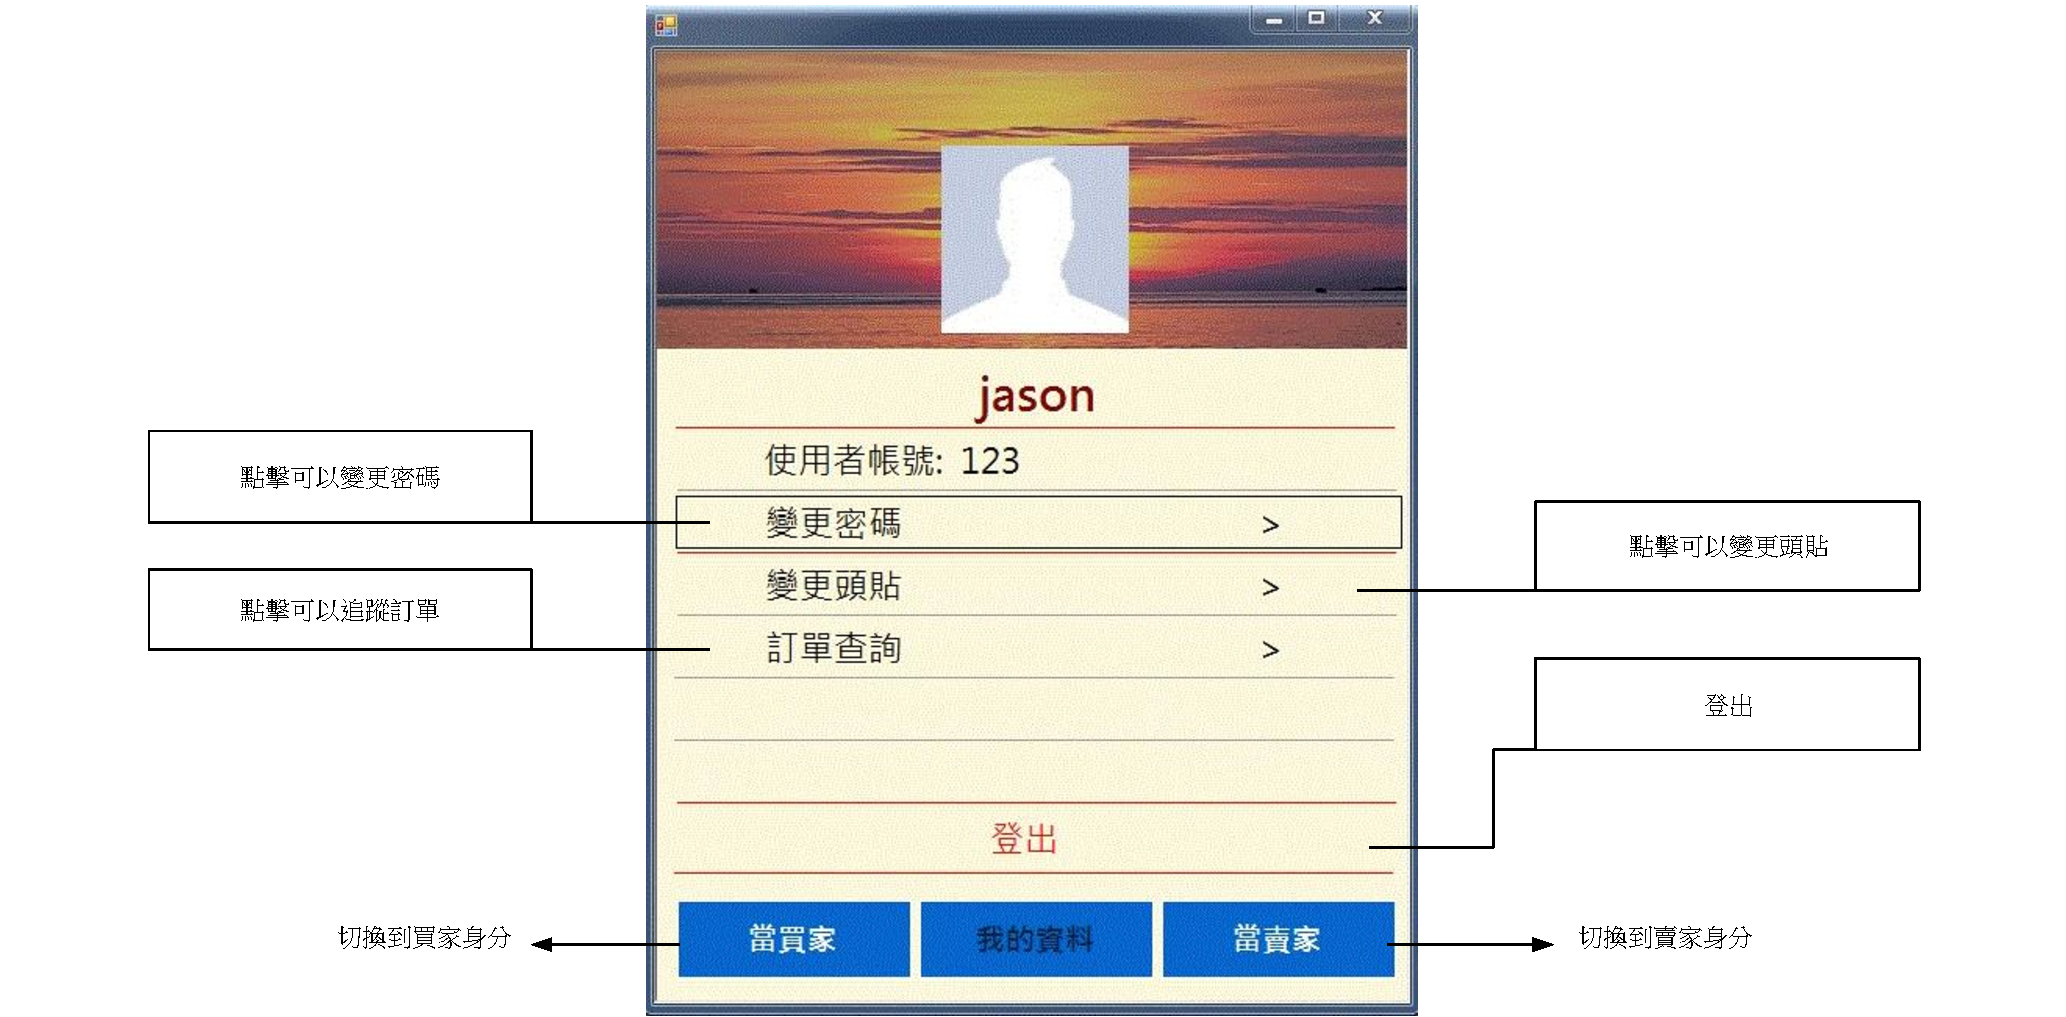
\includegraphics[width=0.95\textwidth]{Info.pdf}
	\caption{使用者的個人資訊。}
\end{figure}

\begin{figure}[t]
	\centering
	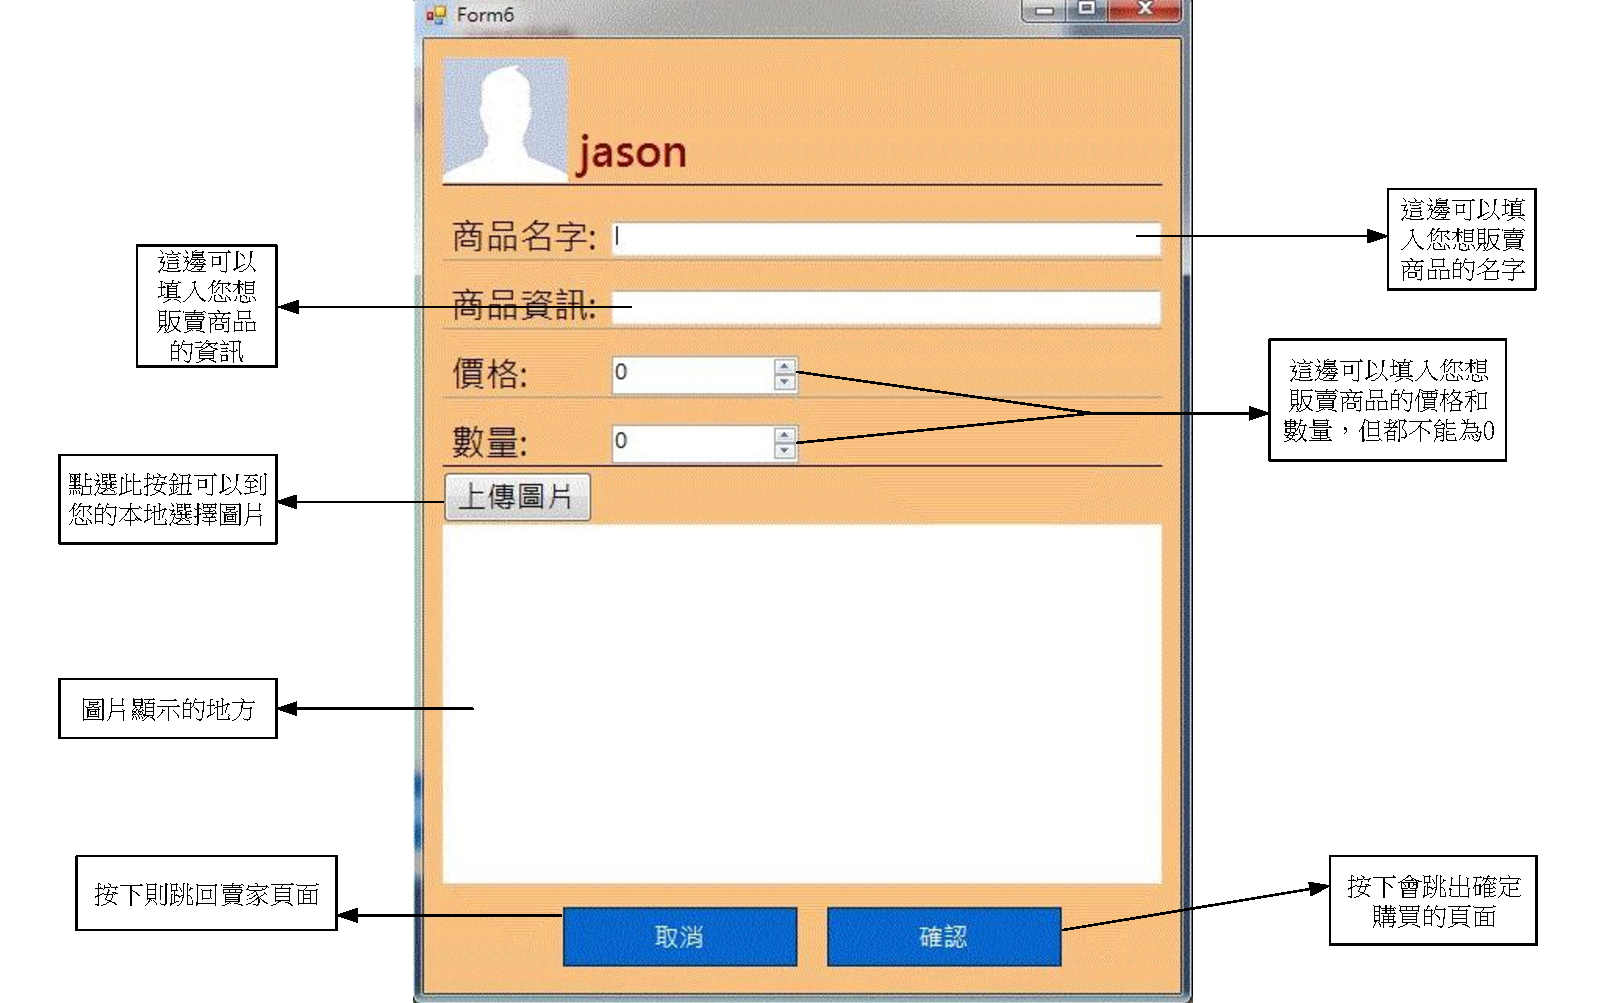
\includegraphics[width=0.85\textwidth]{addpro.pdf}
	\caption{新增商品頁面。}
\end{figure}

\chapter{系統特色}
\section{輕鬆的購物方式}

\subsection{即時性}
\qquad 賣家可以在 FinGer Sopping 隨時新增商品,在有使用者購買其商品時,能提供即時的買賣資訊和通知;買家也可以隨時選取自己想要的商品進行購買,並且即時的追蹤商品的狀態。

\subsection{便利性}
\qquad 在任何有網路的地方,都能隨時當起買家和賣家,只要輕鬆按下一鍵,就能在賣家和買家之間能夠自由切換自己的角色。


\section{舒適的介面}

\subsection{暖色系的色彩}
\qquad 根據研究,由於受到色彩的視覺刺激,而在思維上有所影響。而我們在 FinGer Sopping 上大量採用暖色系的顏料,人類對於暖色系的色彩會感到興奮感,進而提升買家購買的慾望,而對於暖色系的色彩也比較不會對人類的視覺感到疲憊。

\section{產品資訊透明化}
\subsection{評分系統}
\qquad 藉由買家購買的感受度,來給商品評分,讓好的賣家能夠得到更多的回饋,也能讓使用者能夠挑選較優質的商品。

\subsection{留言板的設計}
\qquad 若買家對於商品存在任何疑問,可以透過 FinGer Sopping 提供使用者的留言版來詢問賣家產品的相關問題,也能讓其他想購買此商品的買家能夠在留言板上尋找相關的答案或給予相關的意見。

\chapter{非功能性需求}

\section{安全性}
\qquad 為了保護帳戶安全,存在資料庫當中的密碼會經過SHA-256的計算來確保密碼不會因外洩導致帳號暴露在危險當中。並且使用MongoDB資料庫提供的SSL(傳輸層安全性協定)API建立連結,用以防止資料傳輸安全性的問題,以確保用戶的資料不會外露。

\section{安裝與環境需求}
\qquad 目前提供Windows作業系統,且需要安裝 .NET Framework 4.5.2 或以上版本,加上MongoDB提供的C\#/.NET Driver 2.6的環境下執行。
\chapter{}
\end{CJK}
\end{document}

